\section{Диалоговые системы}

\frame{\tableofcontents[currentsection]}

\begin{frame}
    \frametitle{Отличия от читчата}

    \begin{itemize}
        \item Специфическая доменная область
        \item Дискурсивные ограничения на пользователя
        \item Легко оценить качество
    \end{itemize}
\end{frame}

\begin{frame}
    \frametitle{Фреймы и сценарии}

    \begin{enumerate}
        \item Регистрация в гостинице \begin{itemize}
            \item Участники: клиент, администратор
            \item Действия участников: предъявить, записать, заполнить\ldots
            \item Объекты действия: паспорт, удостоверение личности\ldots
        \end{itemize}
        \item Перемещение по номеру
        \item \ldots
    \end{enumerate}
\end{frame}

\begin{frame}
    \frametitle{Фреймовый подход сегодня}
    \centering
    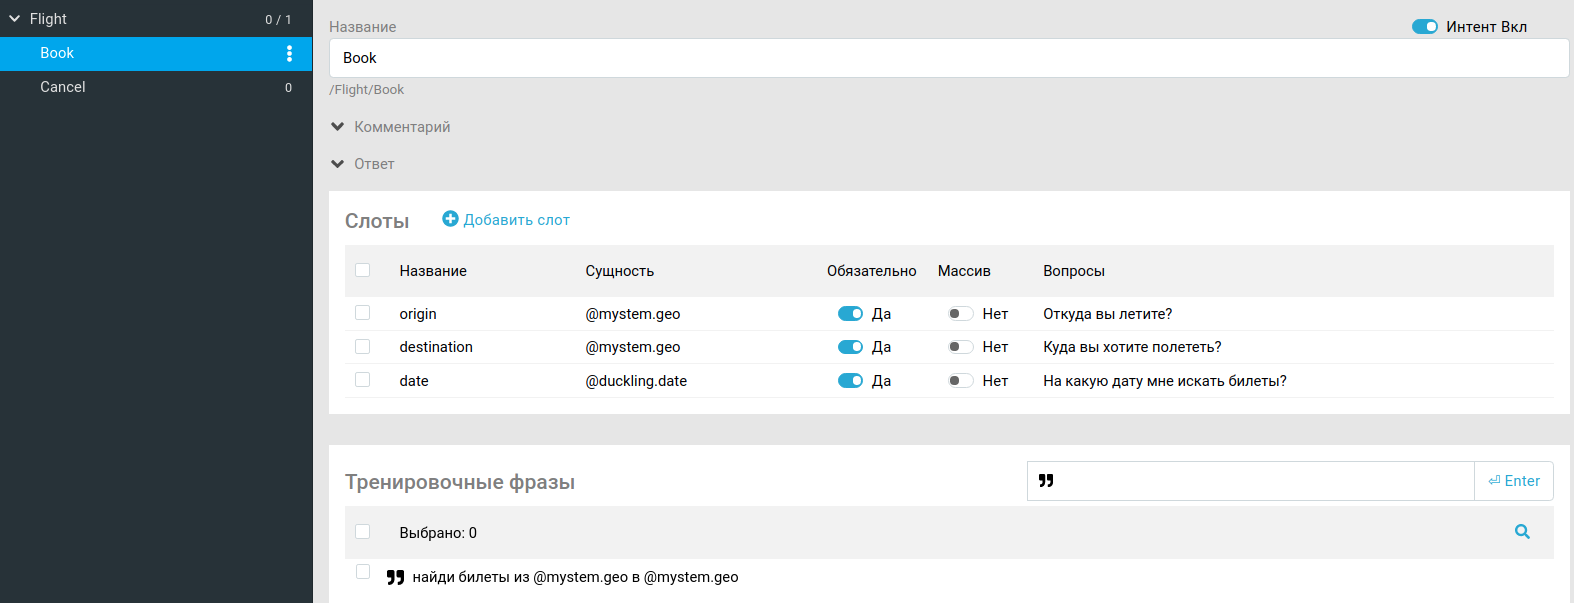
\includegraphics[width=\textwidth]{caila}
\end{frame}

\begin{frame}
    \frametitle{Этапы работы фреймовых диалоговых систем}

    \begin{enumerate}
        \item Определение домена
        \item Определение \textit{интента}
        \item Извлечение \textit{именованных сущностей}
        \item Заполнение \textit{слотов}
        \item Дозаполнение недостающих слотов
        \item Выполнение целевого действия
    \end{enumerate}
\end{frame}

\begin{frame}
    \frametitle{Архитектура диалоговых систем сегодня}
    \centering
    \begin{tikzpicture}[node distance = 5cm]
        \node (asr) {Распознавание речи (ASR)};
        \node (nlu) [right of = asr] {Понимание ЕЯ (NLU)} edge [<-] (asr);
        \node (context) [right of = nlu] {Управление контекстом} edge [<-] (nlu);
        \path (context) -- (context);
        \node (policy) [below of = context] {Политика диалога} edge [<-] (context);
        \node (nlg) [left of = policy] {Генерация ответа (NLG)} edge [<-] (policy);
        \node (tts) [left of = nlg] {Синтез речи (TTS)} edge [<-] (nlg);
        \path (asr) edge [<-] (tts);
    \end{tikzpicture}
\end{frame}

\begin{frame}
    \frametitle{CUI Design}

    \begin{itemize}
        \item Избегать длинных предложений
        \item Избегать открытых вопросов и тупиковых высказываний
        \item Не учить пользователя говорить
        \item Персонифицировать общение
        \item Корректно обрабатывать непонимания
    \end{itemize}

    Все это с учетом особенности целевого канала, мультимодальности, целевой аудитории\ldots
\end{frame}

\begin{frame}
    \frametitle{Обработка коммуникативных неудач}

    \begin{itemize}
        \item Куда и когда вы хотите полететь?
        \item Завтра в Шанхай.
    \end{itemize}

    \onslide<1->{
        \begin{alertblock}{Дословный повтор}
            Простите, я не расслышала. Куда и когда вы хотите полететь?
        \end{alertblock}
    }

    \onslide<2->{
        \begin{block}{Частичный дозапрос}
            Извините, не совсем вас поняла. В какой \textit{город} вы полетите?
        \end{block}
    }

    \onslide<3->{
        \begin{exampleblock}{Дозапрос с пресуппозицией}
            Не могли бы вы еще раз назвать город, в который \textit{завтра} полетите?
        \end{exampleblock}
    }
\end{frame}

\begin{frame}
    \frametitle{Технологии}

    \begin{columns}
        \column{.5\textwidth}
        \begin{block}{Платформы / NLU-провайдеры}
            \begin{itemize}
                \item Dialogflow
                \item LUIS
                \item Rasa
                \item JAICP + CAILA
            \end{itemize}
        \end{block}

        \column{.5\textwidth}
        \begin{block}{Языки / Фреймворки}
            \begin{itemize}
                \item AIML
                \item JAICF
            \end{itemize}
        \end{block}
    \end{columns}
\end{frame}

\begin{frame}
    \frametitle{JAICF}
    \centering
    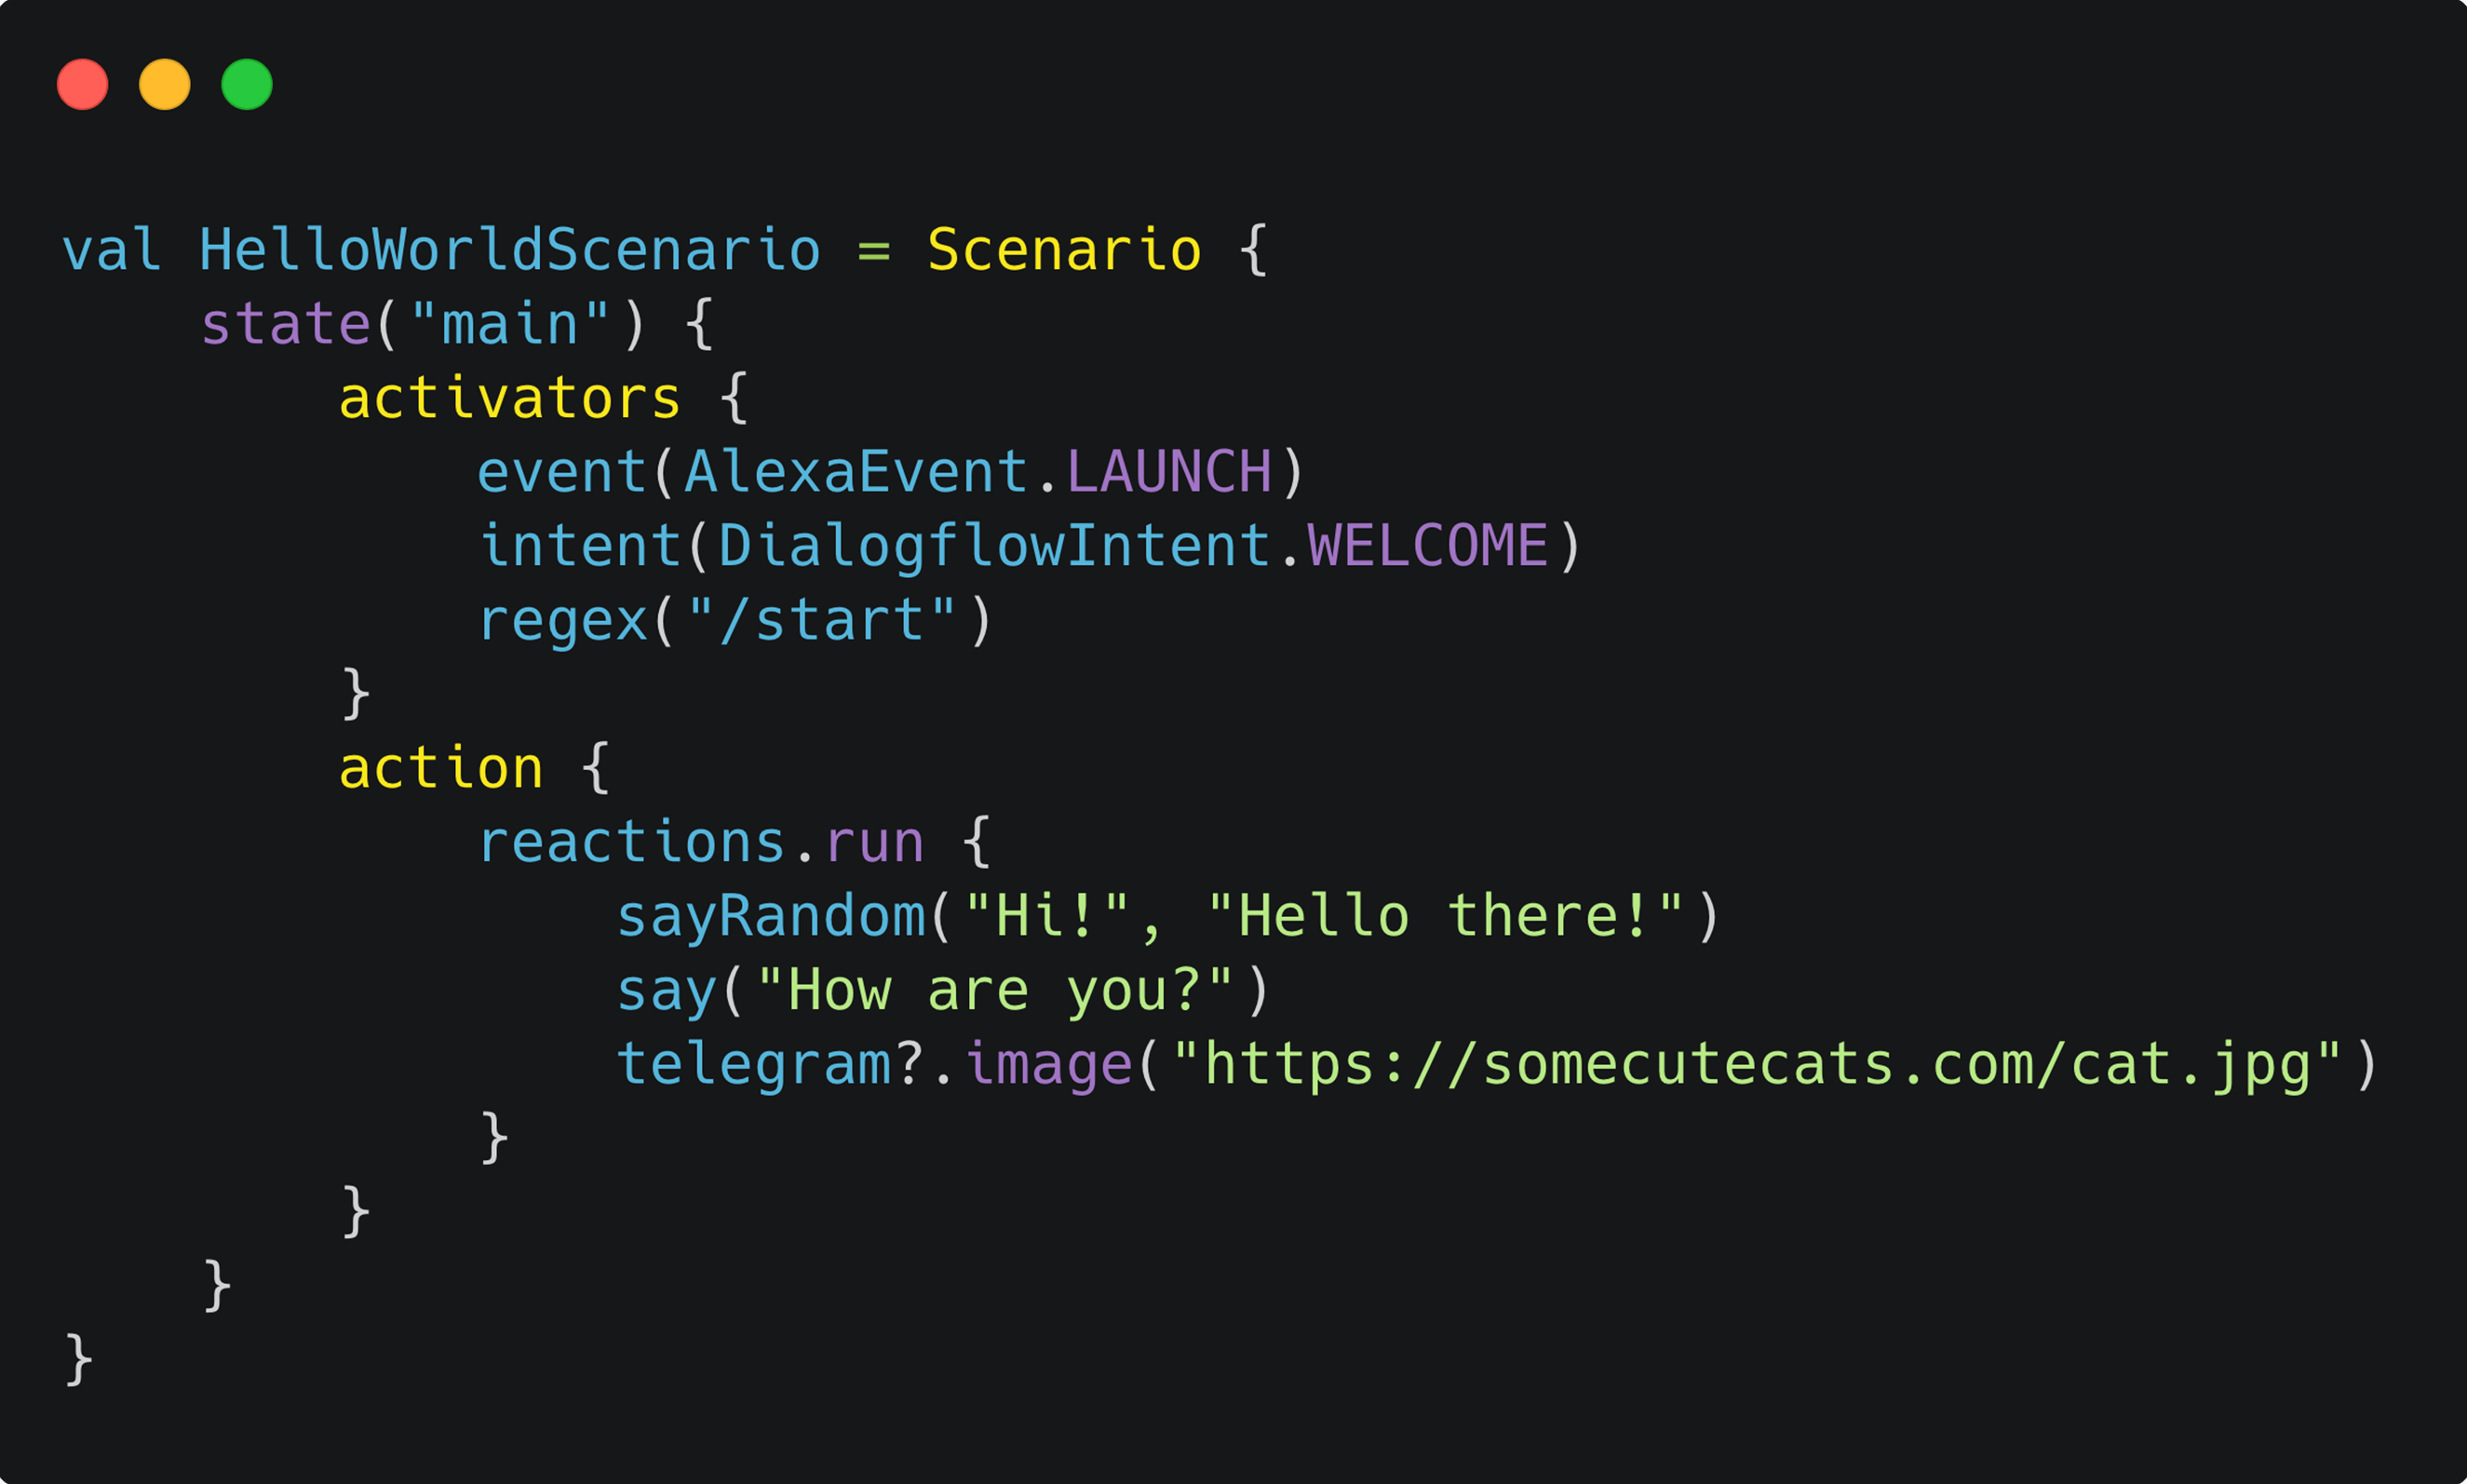
\includegraphics[width=.9\textwidth]{jaicf}
\end{frame}
